\documentclass{article}
\usepackage{amsmath}
\usepackage{amssymb}
\usepackage{amsbsy}
\usepackage{bbm}
\usepackage{url}
\usepackage{color}
\usepackage{float}
\usepackage{graphicx}
\usepackage{epstopdf}
\usepackage{fancyhdr}
\usepackage{enumerate}
\usepackage{tikz}
\usepackage[ruled,vlined]{algorithm2e}
\usepackage[colorlinks=true,urlcolor=blue]{hyperref}
\usepackage[utf8]{inputenc}
\numberwithin{figure}{section}

\newcommand{\Solution}[1]{%
	{%
		\medskip
		\color{red}
		\bf $\bigstar$~\sf\textbf{Solution}~$\bigstar$ \sf
		#1
	}
	\bigskip
}


\graphicspath{{assets}{Homework 1/assets/}}

\title{CS224W Homework 1}

\begin{document}
	
	\maketitle
	
	% Last used - Aut2324
	\section{GNN Expressiveness (28 points)}
	
	
	\textbf{For Q1.1, write down number of layers needed. For Q1.2, write down the transition matrix $M$ and the limiting distribution $r$. For Q1.3 and 1.4, write down the transition matrix w.r.t $A$ and $D$. For Q1.5, write down your proof in a few sentences (equations if necessary). For Q1.6, describe the message function, aggregate function, and update rule in a few sentences or equations.}
	
	Graph Neural Networks (GNNs) are a class of neural network architectures used for deep learning on graph-structured data. Broadly, GNNs aim to generate high-quality embeddings of nodes by iteratively aggregating feature information from local graph neighborhoods using neural networks; embeddings can then be used for recommendations, classification, link prediction, or other downstream tasks. Two important types of GNNs are GCNs (graph convolutional networks) and GraphSAGE (graph sampling and aggregation).
	
	Let $G = (V,E)$ denote a graph with node feature vectors $X_u$ for $u \in V$. To generate the embedding for a node $u$, we use the neighborhood of the node as the computation graph. At every layer $l$, for each pair of nodes $u \in V$ and its neighbor $v \in V$, we compute a message function via neural networks, and apply a convolutional operation that aggregates the messages from the node’s local graph neighborhood (Figure \ref{fig:Q4-gnn-architecture}), and updates the node’s representation at the next layer. By repeating this process through $K$ GNN layers, we capture feature and structural information from a node’s local $K$-hop neighborhood. For each of the message computation, aggregation, and update functions, the learnable parameters are shared across all nodes in the same layer.
	
	\begin{figure}[!htb]
		\centering
		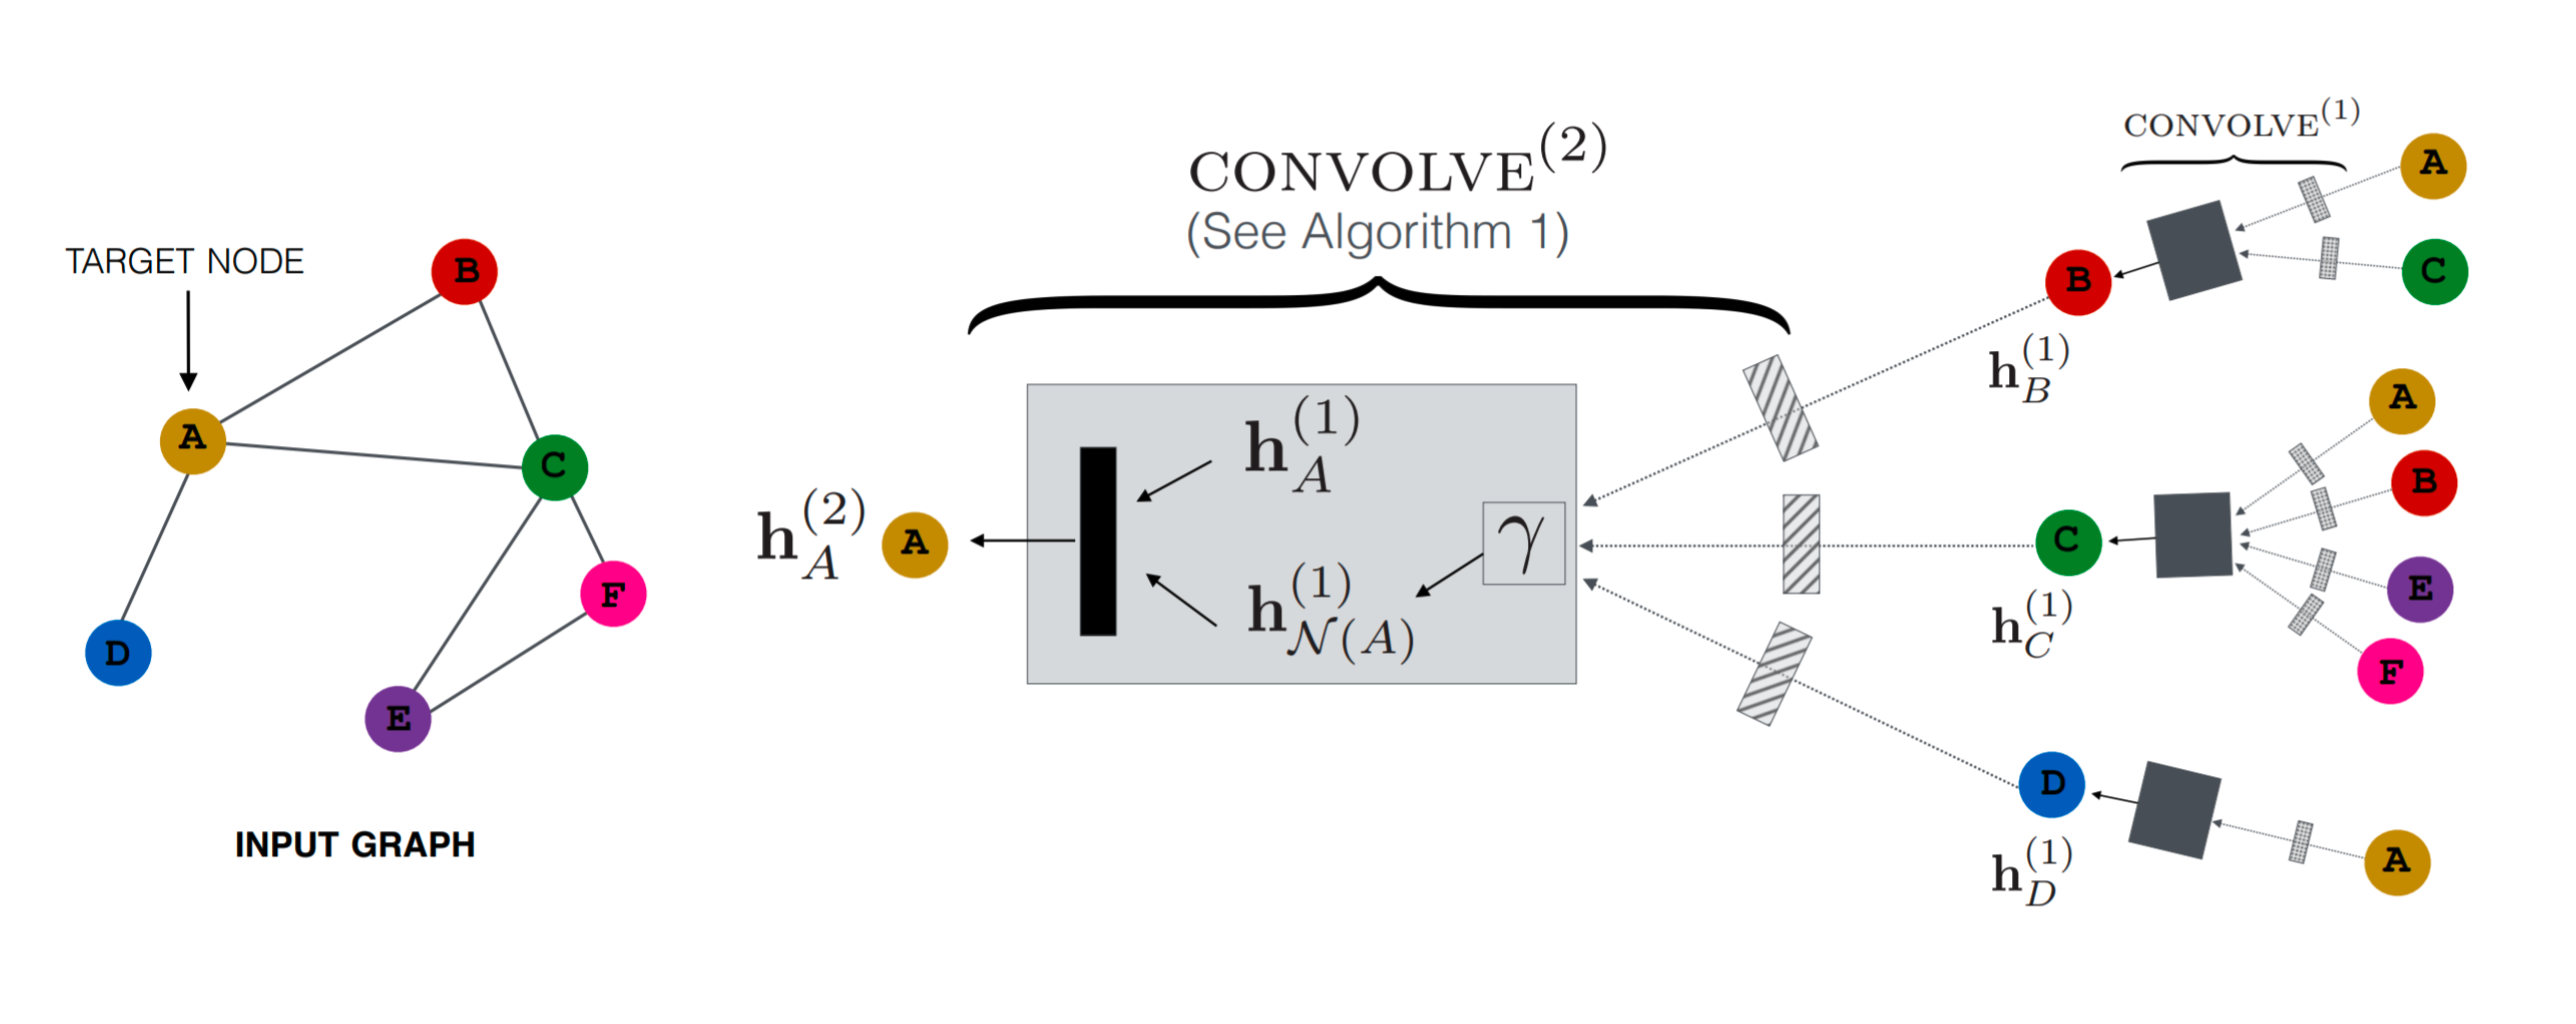
\includegraphics[width=0.7\columnwidth]{gnn-architecture.png}
		\caption{GNN architecture}   
		\label{fig:Q4-gnn-architecture}
	\end{figure}
	
	We initialize the feature vector for node $X_u$ based on its individual node attributes. If we already have outside information about the nodes, we can embed that as a feature vector. Otherwise, we can use a constant feature (vector of 1) or the degree of the node as the feature vector.
	
	These are the key steps in each layer of a GNN:
	\begin{itemize}
		\item \textbf{Message computation}: We use a neural network to learn a message function between nodes. For each pair of nodes $u$ and its neighbor $v$, the neural network message function can be expressed as $M(h^k_u,h^k_v,e_{u,v})$. In GCN and GraphSAGE, this can simply be $\sigma(W h_v + b)$, where $W$ and $b$ are the weights and bias of a neural network linear layer. Here $h^k_u$ refers to the hidden representation of node $u$ at layer $k$, and $e_{u,v}$ denotes available information about the edge $(u, v)$, like the edge weight or other features. For GCN and GraphSAGE, the neighbors of $u$ are simply defined as nodes that are connected to $u$. However, many other variants of GNNs have different definitions of neighborhood.
		\item \textbf{Aggregation}: At each layer, we apply a function to aggregate information from all of the neighbors of each node. The aggregation function is usually permutation invariant, to reflect the fact that nodes’ neighbors have no canonical ordering. In a GCN, the aggregation is done by a weighted sum, where the weight for aggregating from $v$ to $u$ corresponds to the $(u,v)$ entry of the normalized adjacency matrix $D^{-1/2}AD^{-1/2}$.
		\item \textbf{Update}: We update the representation of a node based on the aggregated representation of the neighborhood. For example, in GCNs, a multi-layer perceptron (MLP) is used; Graph-SAGE combines a skip layer with the MLP.
		\item \textbf{Pooling}: The representation of an entire graph can be obtained by adding a pooling layer at the end. The simplest pooling methods are just taking the mean, max, or sum of all of the individual node representations. This is usually done for the purposes of graph classification.
	\end{itemize}
	
	We can formulate the Message computation, Aggregation, and Update steps for a GCN as a layer-wise propagation rule given by:
	\begin{equation}
		h^{k+1} = \sigma(D^{-1/2} A D^{-1/2} h^k W^k)
	\end{equation}
	
	where $h^k$ represents the matrix of activations in the $k$-th layer, $D^{-1/2}AD^{-1/2}$ is the normalized adjacency of graph $G$, $W_k$ is a layer-specific learnable matrix, and $\sigma$ is a non-linearity function. Dropout and other forms of regularization can also be used.
	
	We provide the pseudo-code for GraphSAGE embedding generation below. This will also be relevant to the questions below.
	
	\begin{figure}[H]
		\centering
		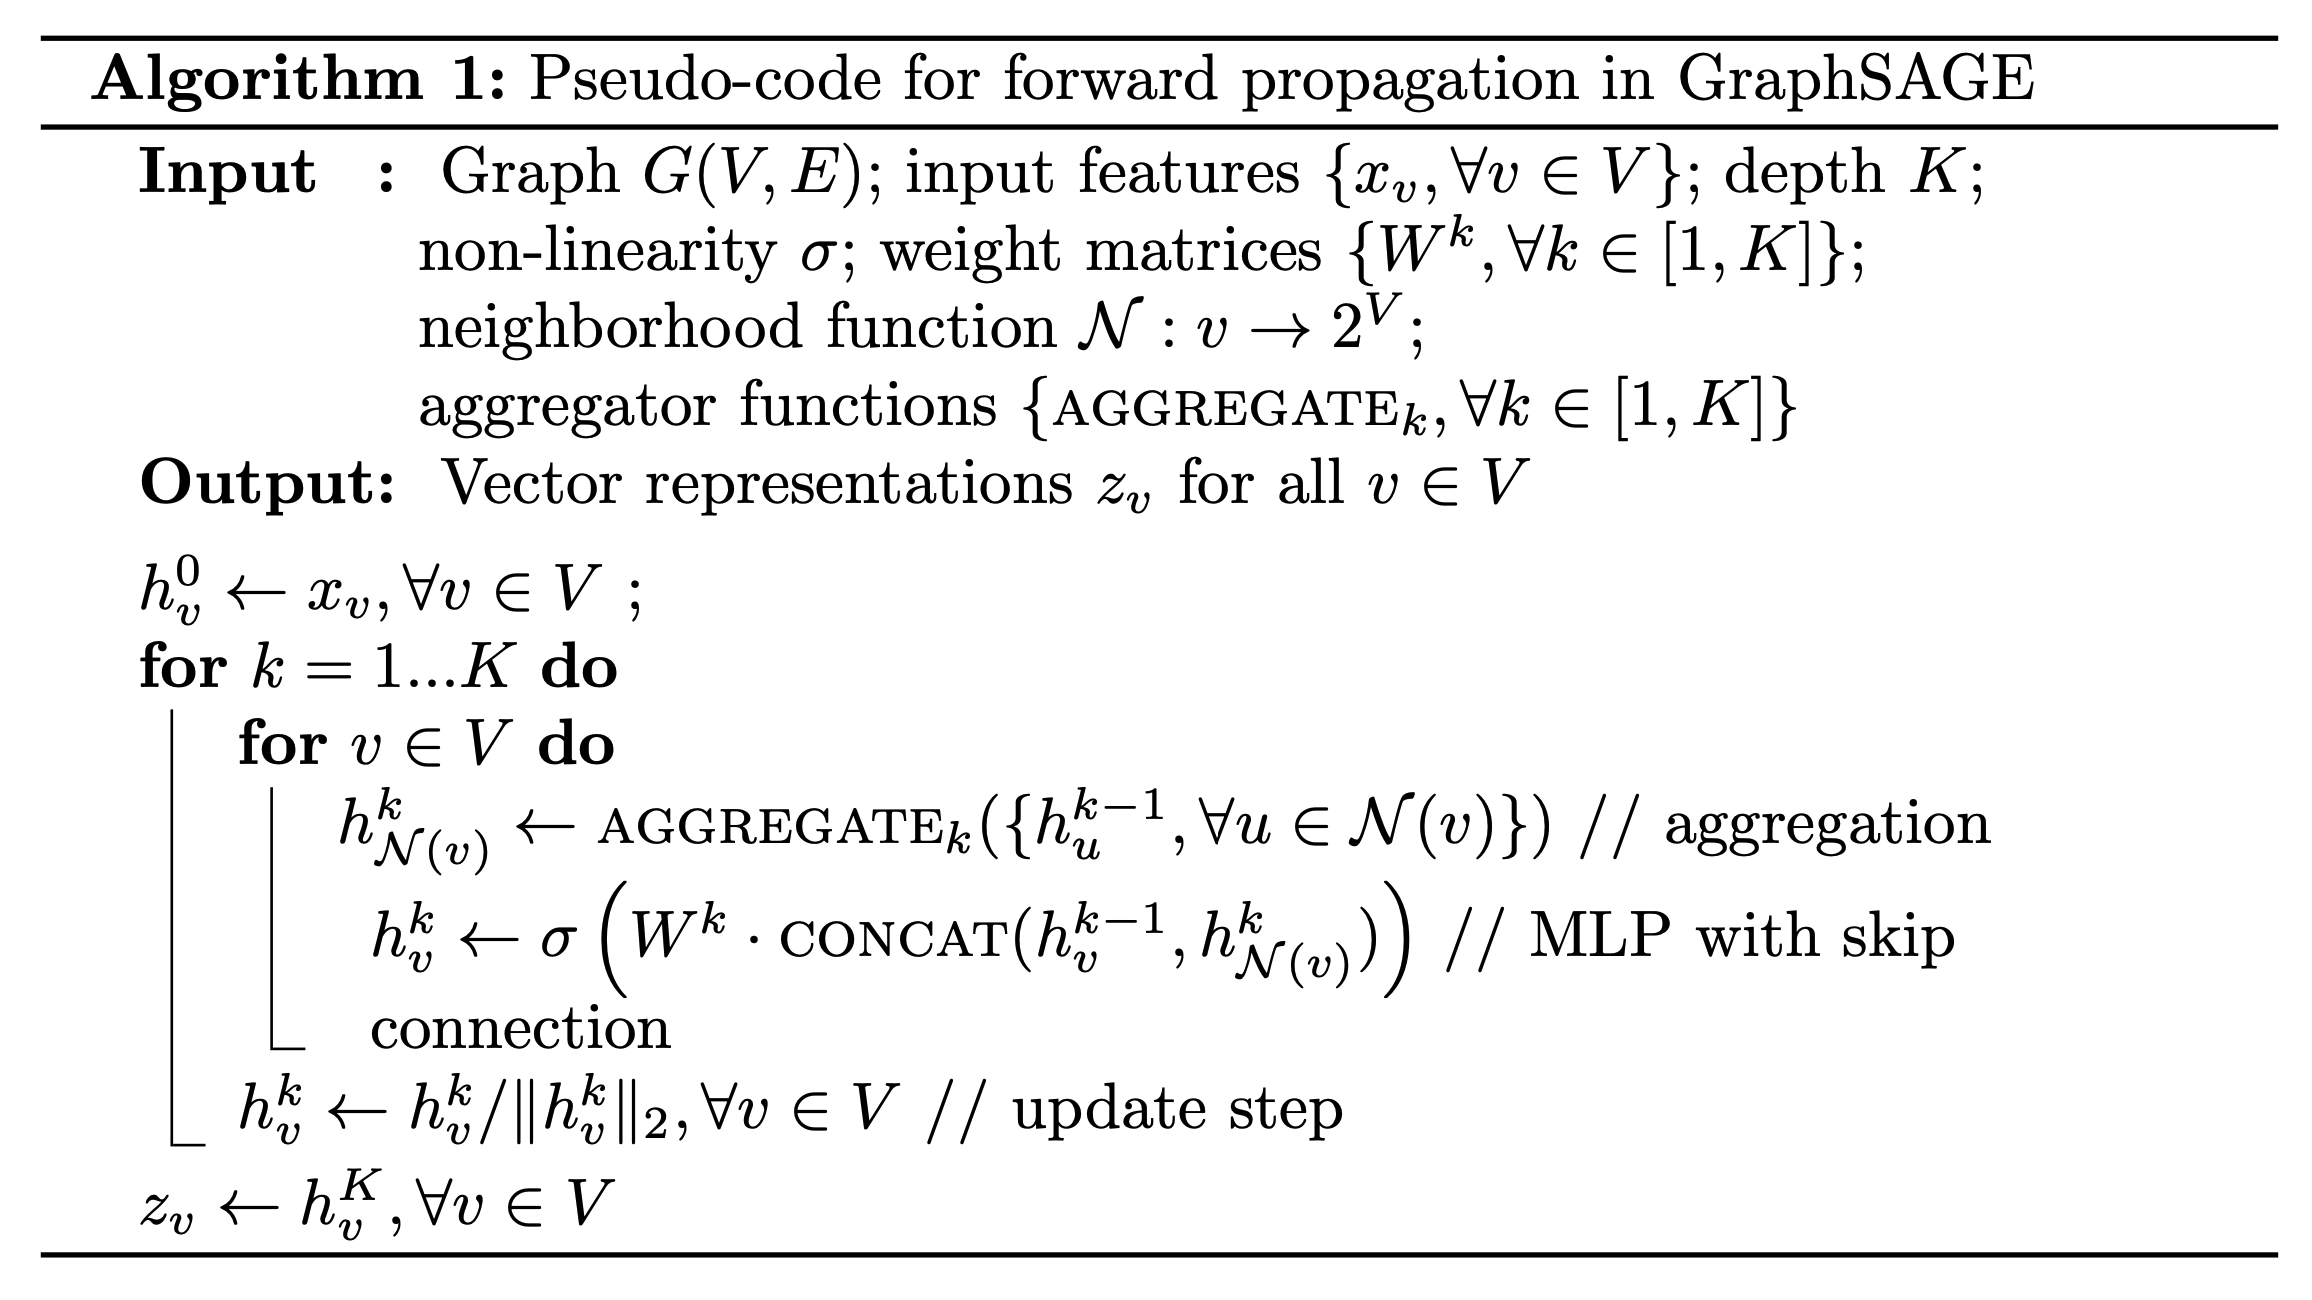
\includegraphics[width=1\columnwidth]{algorithm.png}
	\end{figure}
	
	In this question, we investigate the effect of the number of message passing layers on the expressive power of Graph Convolutional Networks. In neural networks, expressiveness refers to the set of functions (usually the loss function for classification or regression tasks) a neural network is able to compute, which depends on the structural properties of a neural network architecture.
	
	.\\\\
	\subsection{Effect of Depth on Expressiveness (4 points)}
	
	Consider the following 2 graphs in figure~\ref{fig:Q4.1}, where all nodes have 1-dimensional initial feature vector $x = [1]$. We use a simplified version of GNN, with no nonlinearity,
	no learned linear transformation, and sum aggregation. Specifically, at every
	layer, the embedding of node $v$ is updated as the sum over the embeddings of
	its neighbors ($N_v$) and its current embedding $h^t_v$ to get $h^{t+1}_v$. We run the GNN
	to compute node embeddings for the 2 red nodes respectively. Note that the 2 red nodes have different 5-hop neighborhood structure (note this is not the minimum number of hops for which the neighborhood structure of the 2 nodes differs). How many layers of message passing are needed so that these 2 nodes can be distinguished (i.e., have different GNN embeddings)? Explain your answer in a few sentences.
	\\\\\\\\
	\begin{figure}[!htb]
		\centering
		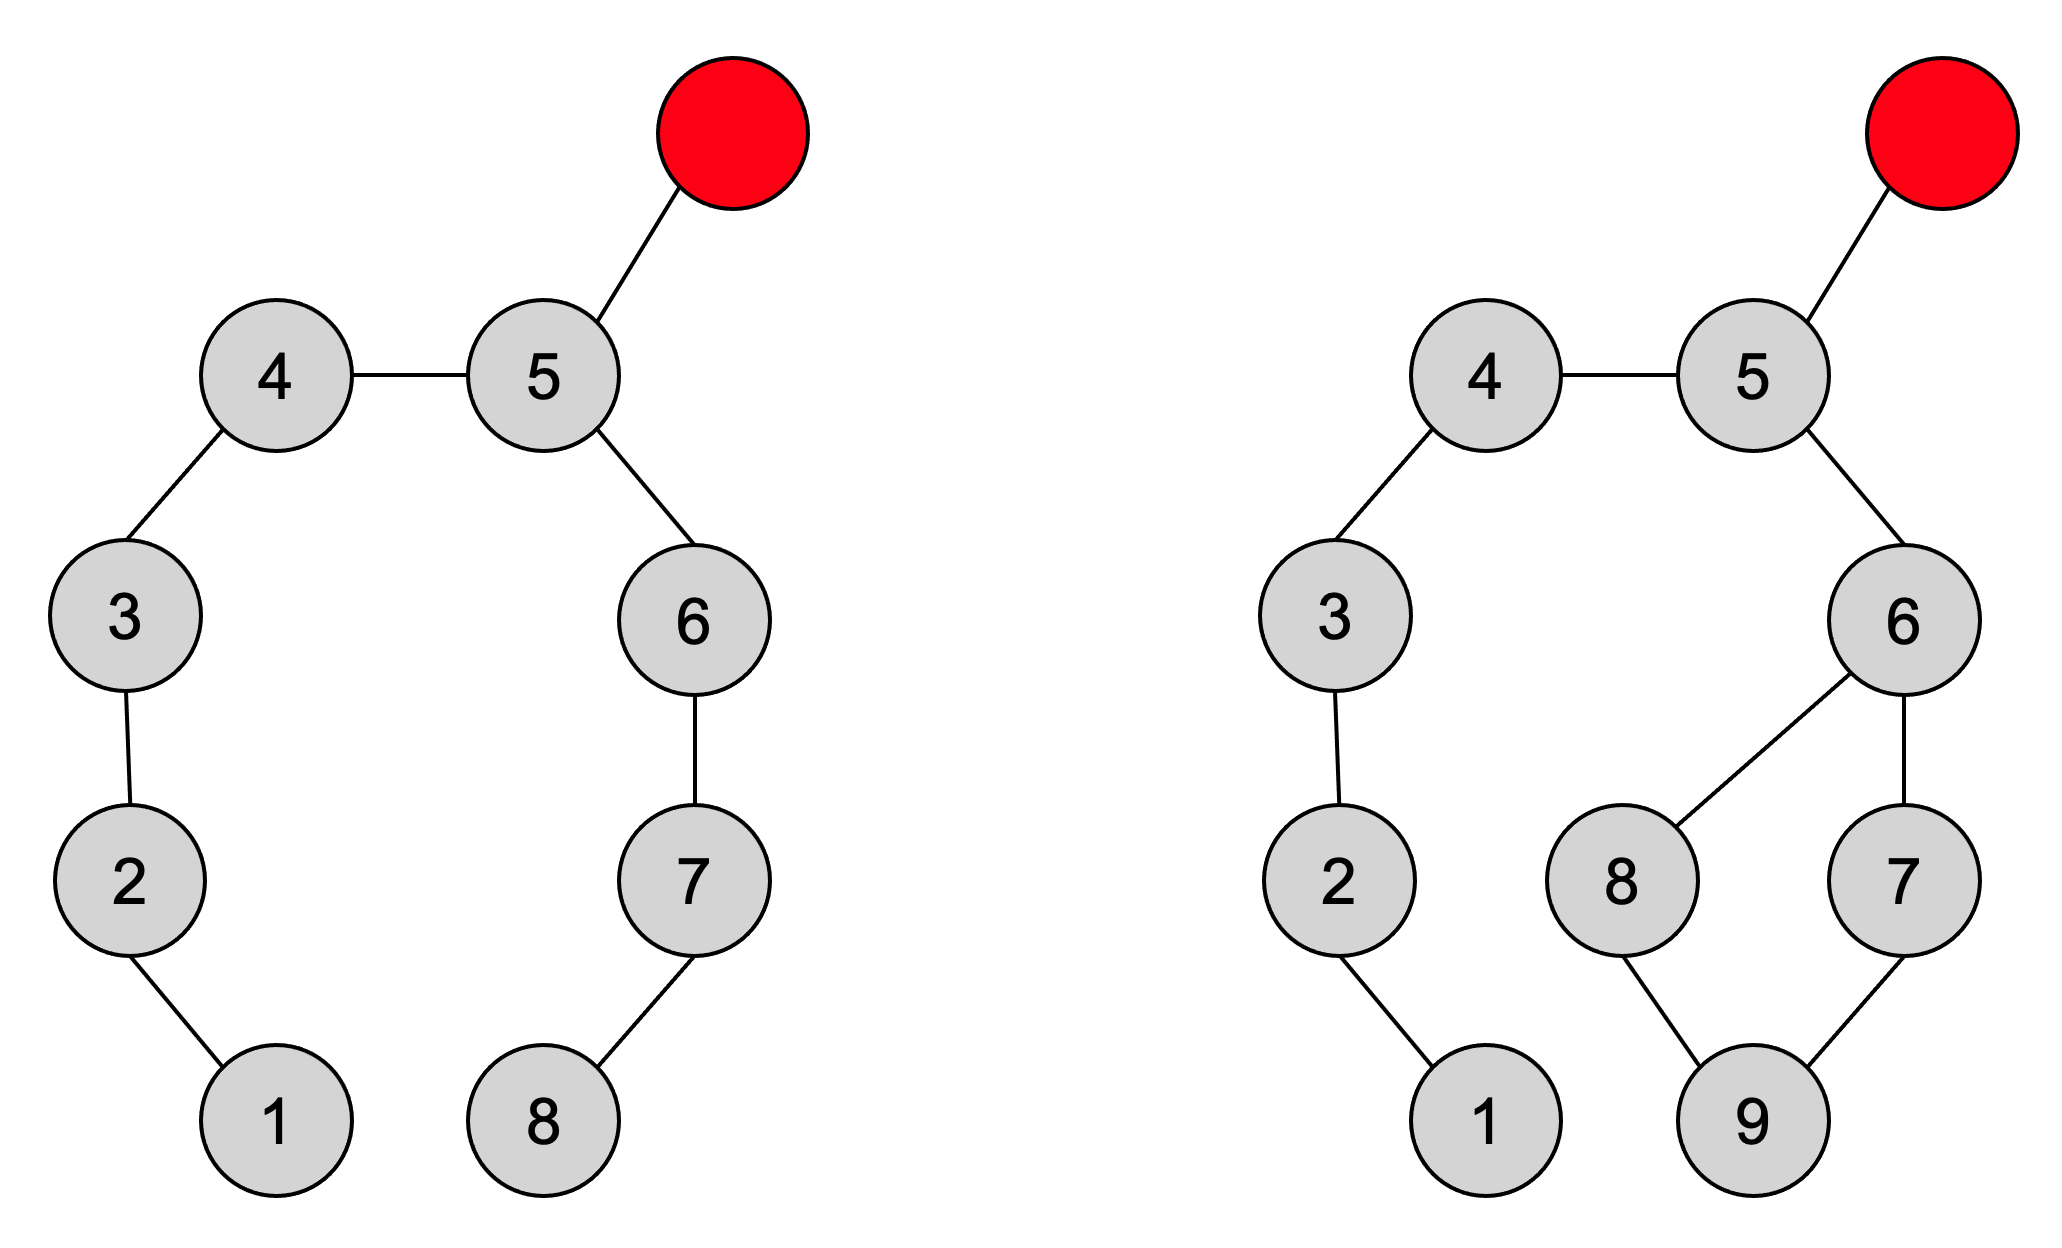
\includegraphics[width=0.6\columnwidth]{fig4-1.png}
		\caption{Figure for Question 1.1}
		\label{fig:Q4.1}
	\end{figure}
	
	.\\
	
	
	\Solution{
		\textbf{3 layers} of message passing are needed.
		\\\\
		\textbf{Explanation:}
		Let's denote the embedding of a node $v$ at layer $t$ as $h^t_v$. The initial embeddings are $h^0_v = 1$ for all nodes $v$ in both graphs. The update rule is given by $h^{t+1}_v = h^t_v + \sum_{u \in N_v} h^t_u$. Let's call the left graph $G_A$ and the right graph $G_B$. We will compute the embeddings for the red node ($v_r$) in both graphs at each layer.
		
		\begin{itemize}
			\item \textbf{Layer 0:} The initial embeddings are identical.
			\\ $h^0_{r, G_A} = 1$
			\\ $h^0_{r, G_B} = 1$
			\\ The embeddings are the same.
			
			\item \textbf{Layer 1:} The red node aggregates from its own $h^0$ and its neighbor's $h^0$ (node 5). The 1-hop neighborhood is identical in both graphs.
			\\ $h^1_{r, G_A} = h^0_{r, G_A} + h^0_{5, G_A} = 1 + 1 = 2$
			\\ $h^1_{r, G_B} = h^0_{r, G_B} + h^0_{5, G_B} = 1 + 1 = 2$
			\\ The embeddings are still the same.
			
			\item \textbf{Layer 2:} The new embedding $h^2_r$ is calculated using $h^1_r$ and the embedding of its neighbor, $h^1_5$.
			\\ To find $h^2_r$, we first need to compute $h^1_5$. In both graphs, the neighbors of node 5 are the red node, node 4, and node 6.
			\\ $h^1_{5, G_A} = h^0_5 + (h^0_r + h^0_4 + h^0_6) = 1 + (1+1+1) = 4$
			\\ $h^1_{5, G_B} = h^0_5 + (h^0_r + h^0_4 + h^0_6) = 1 + (1+1+1) = 4$
			\\ Now, we can compute $h^2_r$ for both graphs:
			\\ $h^2_{r, G_A} = h^1_{r, G_A} + h^1_{5, G_A} = 2 + 4 = 6$
			\\ $h^2_{r, G_B} = h^1_{r, G_B} + h^1_{5, G_B} = 2 + 4 = 6$
			\\ The embeddings are still identical because the 2-hop neighborhood structure is the same.
			
			\item \textbf{Layer 3:} The new embedding $h^3_r$ is calculated using $h^2_r$ and $h^2_5$. The calculation for $h^2_5$ will finally reveal the structural difference between the graphs.
			\\ The computation of $h^2_5$ depends on the $h^1$ embeddings of its neighbors (r, 4, 6). The crucial difference lies in computing $h^1_6$:
			\\ For $G_A$, neighbors of node 6 are \{5, 7\}: $h^1_{6, G_A} = h^0_6 + (h^0_5 + h^0_7) = 1 + (1+1) = 3$.
			\\ For $G_B$, neighbors of node 6 are \{5, 7, 8\}: $h^1_{6, G_B} = h^0_6 + (h^0_5 + h^0_7 + h^0_8) = 1 + (1+1+1) = 4$.
			\\ Now we can compute $h^2_5$. For both graphs, $h^1_r=2$ and $h^1_4 = h^0_4 + (h^0_3+h^0_5) = 1+(1+1)=3$.
			\\ $h^2_{5, G_A} = h^1_5 + (h^1_r + h^1_4 + h^1_{6, G_A}) = 4 + (2 + 3 + 3) = 12$.
			\\ $h^2_{5, G_B} = h^1_5 + (h^1_r + h^1_4 + h^1_{6, G_B}) = 4 + (2 + 3 + 4) = 13$.
			\\ Finally, we can calculate the layer 3 embeddings for the red node:
			\\ $h^3_{r, G_A} = h^2_{r, G_A} + h^2_{5, G_A} = 6 + 12 = \mathbf{18}$
			\\ $h^3_{r, G_B} = h^2_{r, G_B} + h^2_{5, G_B} = 6 + 13 = \mathbf{19}$
			\\ The embeddings are now different.
		\end{itemize}
		The two red nodes can be distinguished after 3 layers. This is because the minimum number of hops required to reach a structural difference from the red node is 3 (the path red $\rightarrow$ 5 $\rightarrow$ 6 $\rightarrow$ 8, which exists only in the right graph). It takes 3 message passing steps for this structural information to propagate to the red node and produce a different embedding.
	}
	
	\subsection{Random Walk Matrix (4 points)}
	
	Consider the graph shown below (figure~\ref{fig:Q4.2}).
	\begin{enumerate}
		\item Assume that the current distribution over nodes is $r = [0,0,1,0]$, and after the random walk, the distribution is $M \cdot r$. What is the random walk transition matrix $M$, where each row of $M$ corresponds with the node ID in the graph?
		\item What is the limiting distribution $r$, namely the eigenvector of $M$ that has an eigenvalue of 1 ($r = Mr$)? Write your answer in fraction form or round it to the nearest thousandth place and in the following form, e.g. $[1.200, 0.111, 0.462, 0.000]$. Note that before reporting you should normalize $r$. \textbf{Hint: $r$ is a probability distribution representing the random walk probabilities for each node after a large number of timesteps}.
	\end{enumerate}
	
	\begin{figure}[!htb]
		\centering
		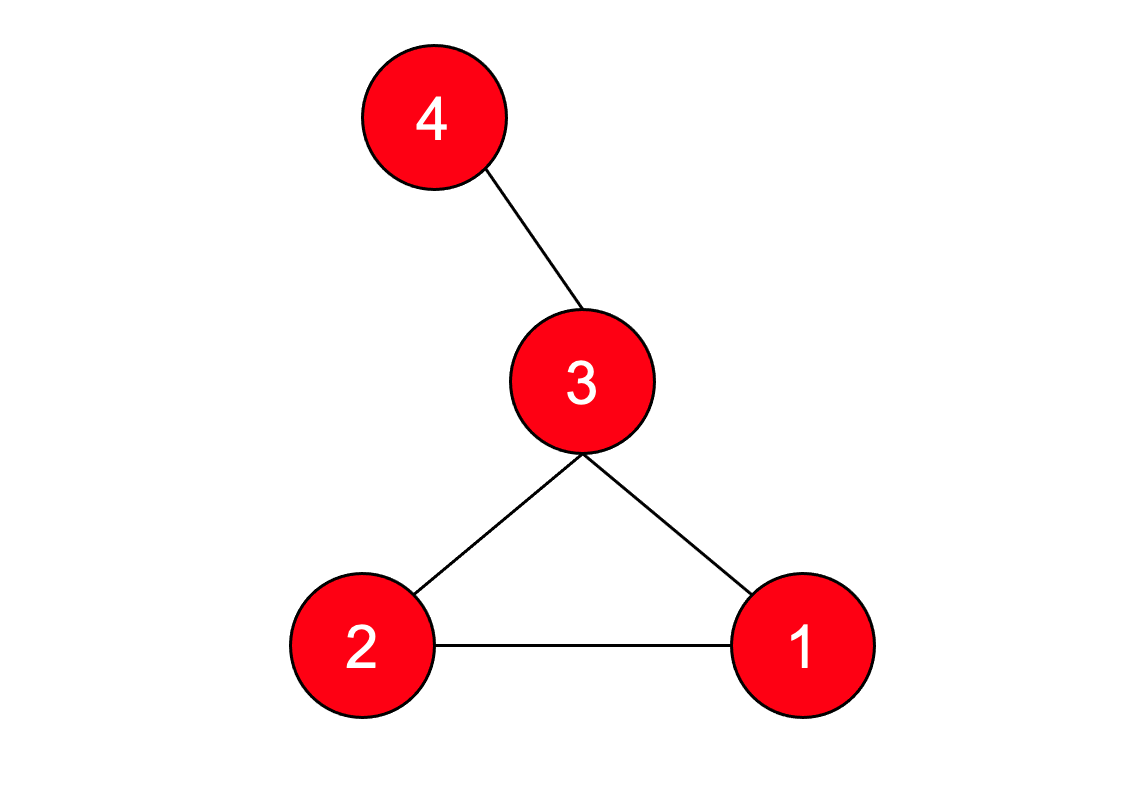
\includegraphics[width=0.5\columnwidth]{fig4-2.png}
		\caption{Figure for Question 1.2}
		\label{fig:Q4.2}
	\end{figure}
	
	\Solution{
		\begin{enumerate}
			\item \textbf{The random walk transition matrix M is:}
			
			The entry $M_{ij}$ of the transition matrix represents the probability of moving from node $j$ to node $i$ in a single step. For an unweighted, undirected graph, this probability is $1/d_j$ if there is an edge between $i$ and $j$ (where $d_j$ is the degree of node $j$), and 0 otherwise. The columns of the matrix correspond to the starting nodes (1, 2, 3, 4).
			
			First, we determine the degrees of the nodes in the given graph: $d_1=2$, $d_2=2$, $d_3=3$, $d_4=1$.
			
			\begin{itemize}
				\item Column 1 (from Node 1, degree 2): Can go to Node 2 or 3 with probability 1/2 each.
				\item Column 2 (from Node 2, degree 2): Can go to Node 1 or 3 with probability 1/2 each.
				\item Column 3 (from Node 3, degree 3): Can go to Node 1, 2, or 4 with probability 1/3 each.
				\item Column 4 (from Node 4, degree 1): Can only go to Node 3.
			\end{itemize}
			
			This gives the following matrix:
			\[
			M = 
			\begin{pmatrix}
				0 & 1/2 & 1/3 & 0 \\
				1/2 & 0 & 1/3 & 0 \\
				1/2 & 1/2 & 0 & 1 \\
				0 & 0 & 1/3 & 0
			\end{pmatrix}
			\]
			
			\item \textbf{The limiting distribution r is:}
			
			For a random walk on an undirected, connected, and non-bipartite graph, the limiting (or stationary) distribution $r$ gives the probability of being at each node after a very large number of steps. The probability for any node $v$, $r_v$, is proportional to its degree $d_v$. It is calculated by the formula:
			\[ r_v = \frac{d_v}{\sum_{u \in V} d_u} \]
			The degrees of each node are: $d_1 = 2$, $d_2 = 2$, $d_3 = 3$, $d_4 = 1$.
			\\
			The sum of all degrees is $\sum d_u = 2 + 2 + 3 + 1 = 8$.
			\\
			Now we can calculate the probability for each node:
			\begin{itemize}
				\item $r_1 = d_1 / 8 = 2/8 = 1/4$
				\item $r_2 = d_2 / 8 = 2/8 = 1/4$
				\item $r_3 = d_3 / 8 = 3/8$
				\item $r_4 = d_4 / 8 = 1/8$
			\end{itemize}
			The resulting limiting distribution vector is:
			\[ r = [1/4, 1/4, 3/8, 1/8] \]
			In the requested format rounded to the nearest thousandth place:
			\[ r = [0.250, 0.250, 0.375, 0.125] \]
			\end{enumerate}
		}
	
	
	\subsection{Relation to Random Walk (i) (4 points)}
	
	Let’s explore the similarity between message passing and random walks. Let $h^{(l)}_i$ be the embedding of node $i$ at layer $l$. Suppose that we are using a mean aggregator for message passing, and omit the learned linear transformation and non-linearity: $h^{(l+1)}_i = \frac{1}{|N_i|} \sum_{j \in N_i} h^{(l)}_j$. If we start at a node $u$ and take a uniform random walk for 1 step, the expectation over the layer-$l$ embeddings
	of nodes we can end up with is $h^{(l+1)}_u$, exactly the embedding of $u$ in the next GNN layer. What is the transition matrix of the random walk? Describe the transition matrix using the adjacency matrix $A$, and degree matrix $D$, a diagonal matrix where $D_{i,i}$ is the degree of node $i$.
	
	\Solution{
		Let $M$ be the transition matrix for the random walk. The entry $M_{ij}$ represents the probability of transitioning from node $j$ to node $i$ in a single step.
		
		The GNN update rule for a node $u$ is given as a mean aggregation of its neighbors' embeddings:
		\[ h^{(l+1)}_u = \frac{1}{|N_u|} \sum_{j \in N_u} h^{(l)}_j \]
		Since $|N_u|$ is the degree of node $u$, which we denote as $d_u$, this can be written as:
		\[ h^{(l+1)}_u = \frac{1}{d_u} \sum_{j \in N_u} h^{(l)}_j \]
		
		Now, consider a uniform random walk starting at node $u$. The walker moves to any of its neighbors $j \in N_u$ with a probability of $P(u \to j) = \frac{1}{d_u}$. The expected value over the layer-$l$ embeddings of the nodes the walker can land on is calculated as follows:
		\[ E[h^{(l)}] = \sum_{j \in N_u} P(u \to j) \cdot h^{(l)}_j = \sum_{j \in N_u} \frac{1}{d_u} h^{(l)}_j = \frac{1}{d_u} \sum_{j \in N_u} h^{(l)}_j \]
		This shows that the GNN update $h^{(l+1)}_u$ is indeed the expected layer-$l$ embedding after a 1-step random walk from $u$.
		
		To describe the transition matrix $M$ of this random walk, we define the probability $M_{ij}$ of moving from a node $j$ to a node $i$:
		\begin{itemize}
			\item A transition from $j$ to $i$ is possible only if there is an edge between them, which is true if $A_{ij} = 1$ (assuming an undirected graph where $A_{ij} = A_{ji}$).
			\item If we are at node $j$, there are $d_j$ possible neighbors to move to, and each is chosen with probability $1/d_j$.
		\end{itemize}
		Therefore, the transition probability is:
		\[ M_{ij} = \begin{cases} 
			\frac{1}{d_j} & \text{if } (j,i) \in E \\
			0 & \text{otherwise} 
		\end{cases}
		\]
		This can be expressed using the adjacency matrix $A$ as $M_{ij} = \frac{A_{ij}}{d_j}$.
		
		To write this in matrix form, we need to scale each column $j$ of the adjacency matrix $A$ by $1/d_j$. This is achieved by right-multiplying $A$ by the inverse of the degree matrix, $D^{-1}$. The degree matrix $D$ is a diagonal matrix with $D_{jj} = d_j$, so its inverse $D^{-1}$ is a diagonal matrix with $(D^{-1})_{jj} = 1/d_j$.
		
		The resulting transition matrix is:
		\[ M = A D^{-1} \]
	}
	
	
	\subsection{Relation to Random Walk (ii) (4 points)}
	
	Suppose that we add a skip connection to the aggregation from Question 1.3:
	$$h^{(l+1)}_i = \frac{1}{2}h^{(l)}_i + \frac{1}{2}\frac{1}{|N_i|} \sum_{j \in N_i} h^{(l)}_j$$
	What is the new corresponding transition matrix?
	
	\Solution{
		The new GNN update rule with a skip connection is:
		\[ h^{(l+1)}_i = \frac{1}{2}h^{(l)}_i + \frac{1}{2}\frac{1}{|N_i|} \sum_{j \in N_i} h^{(l)}_j \]
		This update rule can be interpreted as the expected embedding of a new random walk. At each step, a walker at node $i$ has two choices:
		\begin{enumerate}
			\item With probability $1/2$, the walker stays at the current node $i$.
			\item With probability $1/2$, the walker moves to a uniformly chosen random neighbor $j \in N_i$. The probability of moving to any specific neighbor $j$ is then $\frac{1}{|N_i|} = \frac{1}{d_i}$.
		\end{enumerate}
		
		We can construct the new transition matrix $M$ based on this interpretation. The entry $M_{ij}$ is the probability of transitioning from node $j$ to node $i$.
		
		\begin{itemize}
			\item \textbf{Off-diagonal entries ($i \neq j$):} For a transition from node $j$ to a different node $i$ to occur, the walker must first choose to move (probability $1/2$) and then specifically choose neighbor $i$ out of $d_j$ neighbors (probability $1/d_j$). This is only possible if an edge exists between $i$ and $j$ ($A_{ij}=1$). Thus, the probability is:
			\[ M_{ij} = \frac{1}{2} \cdot \frac{A_{ij}}{d_j} \quad \text{for } i \neq j \]
			This part of the transition matrix can be written as $\frac{1}{2} A D^{-1}$.
			
			\item \textbf{Diagonal entries ($i = j$):} For a walker to remain at node $j$, it must choose to stay (probability $1/2$). Thus:
			\[ M_{jj} = \frac{1}{2} \]
			This part of the transition matrix corresponds to $\frac{1}{2}I$, where $I$ is the identity matrix.
		\end{itemize}
		
		Combining these two parts, the new transition matrix is the sum of the "staying" matrix and the "moving" matrix:
		\[ M = \frac{1}{2}I + \frac{1}{2} A D^{-1} \]
		We can also factor out the $1/2$ to get:
		\[ M = \frac{1}{2} (I + A D^{-1}) \]
	}
	
	
	\subsection{Over-Smoothing Effect (5 points)}
	
	In Question 1.1 we see that increasing depth could give more expressive power.
	On the other hand, however, a very large depth also gives rise to the undesirable
	effect of over smoothing. Assume we are still using the aggregation function
	from Question 1.3: $h^{(l+1)}_i = \frac{1}{|N_i|} \sum_{j \in N_i} h^{(l)}_j$. Show that the node embedding $h^{(l)}$ will converge as $l \rightarrow \infty$. Here we assume that the graph is connected and has no bipartite components. We also assume that the graph is undirected.
	
	Over-smoothing thus refers to the problem of node embedding convergence. Namely, if all node embeddings converge to the same value then we can no longer distinguish them and our node embeddings become useless for downstream tasks. However, in practice, learnable weights, non-linearity, and other architecture choices can alleviate the over-smoothing effect.
	
	\textbf{Hint: Here are some properties that might be helpful: 
		\begin{itemize}
			\item A Markov Chain is \textit{irreducible} if every state can be reached from every other state. 
			\item A state $i$ of a Markov Chain is \textit{periodic} if, for a certain $t>1$, it is only possible to travel from $i$ to $i$ in multiples of $t$ timesteps. A Markov Chain is \textit{aperiodic} if it has no periodic states. 
			\item If a Markov Chain is irreducible and aperiodic, it will converge to a unique stationary distribution regardless of the starting state. 
		\end{itemize} You don’t need to be super rigorous with your proof.}
	
	\Solution{
		We can demonstrate the convergence of node embeddings by interpreting the GNN's layer-wise updates as a power iteration on a transition matrix from a random walk.
		
		1.  \textbf{Matrix Formulation of the GNN Update:}
		The given aggregation function is $h^{(l+1)}_i = \frac{1}{|N_i|} \sum_{j \in N_i} h^{(l)}_j$. Let $h^{(l)}$ be the matrix of all node embeddings at layer $l$. This update rule can be expressed in matrix form as:
		\[ h^{(l+1)} = D^{-1}A h^{(l)} \]
		where $A$ is the adjacency matrix and $D$ is the diagonal degree matrix. Let's define the transition matrix $P = D^{-1}A$. Repeated application of this rule gives:
		\[ h^{(l)} = (D^{-1}A)^l h^{(0)} = P^l h^{(0)} \]
		The behavior of the embeddings $h^{(l)}$ as $l \rightarrow \infty$ is determined by the limit of the matrix power $P^l$.
		
		2.  \textbf{Connection to Markov Chains:}
		The matrix $P$ is the transition matrix of a random walk on the graph. The problem provides assumptions about the graph that correspond to key properties of this Markov Chain:
		\begin{itemize}
			\item The graph is \textbf{connected}, which means the corresponding Markov Chain is \textbf{irreducible}. Every node can be reached from every other node.
			\item The graph has \textbf{no bipartite components}, which means the Markov Chain is \textbf{aperiodic}.
		\end{itemize}
		
		3.  \textbf{Convergence to a Stationary Distribution:}
		According to the fundamental theorem of regular Markov Chains (which are irreducible and aperiodic), as $l \rightarrow \infty$, the matrix $P^l$ converges to a limiting matrix $P_\infty$. This matrix $P_\infty$ has the property that all of its rows are identical and equal to the unique stationary distribution vector $\pi^T$.
		\[ \lim_{l\to\infty} P^l = P_\infty = \mathbf{1} \pi^T = 
		\begin{pmatrix}
			- & \pi^T & - \\
			- & \pi^T & - \\
			& \vdots & \\
			- & \pi^T & -
		\end{pmatrix}
		\]
		For a random walk on an undirected graph, the stationary probability $\pi_j$ of being at node $j$ is proportional to its degree $d_j$:
		\[ \pi_j = \frac{d_j}{\sum_{k \in V} d_k} = \frac{d_j}{2|E|} \]
		
		4.  \textbf{Resulting Node Embeddings:}
		Now, we can find the final node embeddings by applying the limiting matrix $P_\infty$ to the initial embeddings $h^{(0)}$:
		\[ h^{(\infty)} = \lim_{l\to\infty} h^{(l)} = P_\infty h^{(0)} \]
		Let's examine the embedding for an arbitrary node $i$, which is the $i$-th row of the resulting vector:
		\[ h^{(\infty)}_i = (P_\infty h^{(0)})_i = \sum_{j \in V} (P_\infty)_{ij} h^{(0)}_j \]
		Since every row of $P_\infty$ is $\pi^T$, we have $(P_\infty)_{ij} = \pi_j$ for all $i$. Therefore:
		\[ h^{(\infty)}_i = \sum_{j \in V} \pi_j h^{(0)}_j = \sum_{j \in V} \frac{d_j}{2|E|} h^{(0)}_j \]
		The final expression is a constant value—a weighted average of the initial node features, where the weights are determined by the stationary distribution. This value is independent of the node $i$. Therefore, as $l \rightarrow \infty$, the embeddings of all nodes converge to the exact same value. This loss of distinctiveness between nodes is the over-smoothing effect.
	}
	
	
	\subsection{Learning BFS with GNN (7 points)}
	
	Next, we investigate the expressive power of GNN for learning simple graph algorithms. Consider breadth-first search (BFS), where at every step, nodes that are connected to already visited nodes become visited. Suppose that we use GNN to learn to execute the BFS algorithm. Suppose that the embeddings are 1-dimensional. Initially, all nodes have input feature 0, except a source node which has input feature 1. At every step, nodes reached by BFS have embedding 1, and nodes not reached by BFS have embedding 0. Describe a message function, an aggregation function, and an update rule for the GNN such that it learns the task perfectly.
	
	\Solution{
		To perfectly learn the BFS algorithm, the GNN must be able to propagate a "visited" status from a node to its neighbors at each layer, ensuring that once a node is visited, it remains visited. Let $h_v^{(k)}$ be the 1-dimensional embedding of node $v$ at layer $k$, where $h_v^{(k)}=1$ if the node has been reached by the BFS and $h_v^{(k)}=0$ otherwise.
		
		The initial state is $h_{\text{source}}^{(0)} = 1$ and $h_v^{(0)} = 0$ for all other nodes $v$. The GNN components can be defined as follows:
		
		\begin{itemize}
			\item \textbf{Message Function:} Each node $v$ simply passes its current state (embedding) as the message to its neighbors.
			\[ \text{Message}(h_v^{(k)}) = h_v^{(k)} \]
			This means a node sends a `1` if it is currently "visited" and a `0` otherwise.
			
			\item \textbf{Aggregation Function:} A node $u$ aggregates the messages from its neighbors $v \in N_u$ by taking the maximum value.
			\[ m_u^{(k)} = \underset{v \in N_u}{\text{MAX}} \left( \text{Message}(h_v^{(k)}) \right) = \underset{v \in N_u}{\text{MAX}} \left( h_v^{(k)} \right) \]
			This aggregation step effectively checks if \textit{at least one} neighbor of $u$ was visited in the previous step. If any neighbor $v$ has $h_v^{(k)}=1$, the aggregated message $m_u^{(k)}$ will be 1; otherwise, it will be 0.
			
			\item \textbf{Update Rule:} A node $u$ updates its embedding for the next layer by taking the maximum of its own current embedding and the aggregated message from its neighbors.
			\[ h_u^{(k+1)} = \text{MAX} \left( h_u^{(k)}, m_u^{(k)} \right) = \text{MAX} \left( h_u^{(k)}, \underset{v \in N_u}{\text{MAX}}(h_v^{(k)}) \right) \]
			This update rule ensures two critical properties of BFS:
			\begin{enumerate}
				\item \textbf{Propagation:} If an unvisited node $u$ ($h_u^{(k)}=0$) is connected to a visited node ($m_u^{(k)}=1$), its new state will be $\text{MAX}(0, 1) = 1$. This mimics the expansion of the BFS frontier.
				\item \textbf{Persistence:} If a node $u$ is already visited ($h_u^{(k)}=1$), its new state will be $\text{MAX}(1, m_u^{(k)}) = 1$, regardless of its neighbors' states. This ensures that a node, once reached, remains "visited" in all subsequent steps.
			\end{enumerate}
		\end{itemize}
		
		With these components, the GNN layer-$k$ embeddings will represent the set of nodes reachable from the source node in $k$ or fewer hops, perfectly simulating the BFS algorithm.
	}
	
	
	
	% Last used - Aut2324
	\section{Node Embedding and its Relation to Matrix Factorization (24 points)}
	
	\textbf{ What to submit: For Q2.1, one or more sentences/equations describing the decoder. For Q2.2, write down the objective function. For Q2.3, describe the characteristics of $W$ in one or more sentences. For Q2.4, write down the objective function. For Q2.5, characterize the embeddings, whether you think it will reflect structural similarity, and your justification. For Q2.6, one or more sentences for node2vec and struct2vec respectively. For Q2.7, one or more sentences of explanation. For Q2.8, one or more sentences characterizing embeddings from struct2vec.}
	
	Recall that matrix factorization and the encoder-decoder view of node embeddings are closely related. For the embeddings, when properly formulating the encoder-decoder and the objective function, we can find equivalent matrix factorization formulation approaches.\\
	\\
	Note that in matrix factorization we are optimizing for L2 distance; in encoder-decoder examples such as DeepWalk and node2vec, we often use log-likelihood as in lecture slides. The goal to approximate A with $Z^TZ$ is the same, but for this question, stick with the L2 objective function.
	\subsection{Simple matrix factorization (3 points)}
	In the simple matrix factorization, the objective is to approximate adjacency matrix A by the product of embedding matrix with its transpose. The optimization objective is $\min_Z ||A - Z^TZ||_2$.\\
	\\
	In the encoder-decoder perspective of node embeddings, what is the decoder? (Please provide a mathematical expression for the decoder)
	
	\Solution{
		In the encoder-decoder framework for node embeddings, the encoder maps each node to a low-dimensional vector (its embedding), and the decoder uses these embeddings to reconstruct the similarity between nodes.
		
		In this specific problem, the objective is to make the reconstructed similarity matrix $Z^TZ$ as close as possible to the adjacency matrix $A$. The encoder is an embedding lookup: for a node $u$, the encoder outputs its embedding vector $z_u$ (the $u$-th row of the matrix $Z$).
		
		The decoder takes the embeddings of two nodes, $u$ and $v$, and outputs a scalar similarity score that should approximate $A_{uv}$. The reconstructed similarity score between nodes $u$ and $v$ is given by the $(u,v)$-th entry of the matrix $Z^TZ$. This entry is calculated as the dot product of the embedding vectors for node $u$ and node $v$.
		
		Therefore, the decoder is the dot product of the node embeddings. The mathematical expression for the decoder is:
		\[ \text{DEC}(z_u, z_v) = z_u^T z_v \]
	}
	
	
	
	\subsection{Alternate matrix factorization (3 points)}
	In linear algebra, we define bilinear form as $z_i^T W z_j$, where W is a matrix. Suppose that we define the decoder as the bilinear form, what would be the objective function for the corresponding matrix factorization? (Assume that the $W$ matrix is fixed)
	
	\Solution{
		The objective function aims to minimize the L2 distance (Frobenius norm) between the true adjacency matrix $A$ and a reconstructed similarity matrix, which we can call $\hat{A}$. The decoder defines how each element of $\hat{A}$ is calculated from the node embeddings.
		
		The new decoder is defined as the bilinear form:
		\[ \text{DEC}(z_i, z_j) = z_i^T W z_j \]
		This means the reconstructed similarity for the node pair $(i, j)$ is $\hat{A}_{ij} = z_i^T W z_j$.
		
		We need to express the entire reconstructed matrix $\hat{A}$ in terms of the embedding matrix $Z$ and the fixed matrix $W$. The $(i,j)$-th element of the matrix product $Z W Z^T$ is computed by taking the $i$-th row of $Z$ (which is $z_i^T$), multiplying by $W$, and then taking the dot product with the $j$-th column of $Z^T$ (which is $z_j$). This gives the expression $z_i^T W z_j$.
		
		Therefore, the full reconstructed matrix is $\hat{A} = Z W Z^T$.
		
		The objective function for the corresponding matrix factorization, which minimizes the L2 norm of the difference between the true and reconstructed matrices, is:
		\[ \min_Z ||A - Z W Z^T||_2 \]
		Since the matrix $W$ is assumed to be fixed, the optimization is performed only over the embedding matrix $Z$.
	}
	
	
	
	\subsection{BONUS: Relation to eigen-decomposition (3 points)}
	Recall eigen-decomposition of a matrix (\href{https://en.wikipedia.org/wiki/Eigendecomposition_of_a_matrix}{link}). What would be the condition of W, such that the matrix factorization in the previous question (2.2) is equivalent to learning the eigen-decomposition of matrix A?
	
	\Solution{
		The objective is for the matrix factorization from Q2.2, which seeks to approximate $A$ with $Z W Z^T$, to be equivalent to the eigen-decomposition of $A$.
		
		First, let's recall the eigen-decomposition of the adjacency matrix $A$. Since the graph is undirected, $A$ is a real, symmetric matrix. A real symmetric matrix can be diagonalized by an orthogonal matrix. Its eigen-decomposition is given by:
		\[ A = Q \Lambda Q^T \]
		where:
		\begin{itemize}
			\item $Q$ is an orthogonal matrix ($Q^T Q = I$) whose columns are the orthonormal eigenvectors of $A$.
			\item $\Lambda$ is a diagonal matrix whose diagonal entries are the corresponding real eigenvalues of $A$.
		\end{itemize}
		
		Now, let's look at the matrix factorization objective from the previous question:
		\[ \min_Z ||A - Z W Z^T||_2 \]
		The goal of this optimization is to find an embedding matrix $Z$ that makes $Z W Z^T$ the best possible approximation of $A$. The problem becomes equivalent to learning the eigen-decomposition if the minimum objective value is zero, which occurs when $A = Z W Z^T$.
		
		By comparing the two forms:
		\[ Z W Z^T = Q \Lambda Q^T \]
		We can see a direct correspondence. If we set the learned embedding matrix $Z$ to be the matrix of orthonormal eigenvectors $Q$, the equation becomes $Q W Q^T = Q \Lambda Q^T$. This implies that $W$ must be equal to $\Lambda$.
		
		Therefore, the condition on $W$ is that it must be a \textbf{diagonal matrix containing the eigenvalues of A} on its diagonal.
	}
	
	\subsection{Multi-hop node similarity (3 points)}
	Define node similarity with the multi-hop definition: 2 nodes are similar if they are connected by at least one path of length at most k, where k is a parameter (e.g. $k = 2$). Suppose that we use the same encoder (embedding lookup) and decoder (inner product) as before. What would be the corresponding matrix factorization problem we want to solve?
	
	\Solution{
		The problem requires us to define a matrix factorization objective where the target is a new multi-hop similarity matrix, let's call it $S$. The encoder (embedding lookup) and decoder (inner product) are the same as in Q2.1, meaning our model will attempt to approximate the target matrix $S$ with the matrix product $Z^TZ$.
		
		The main task is to mathematically define the target similarity matrix $S$. The similarity is defined as: two nodes $u$ and $v$ are similar if there is at least one path of length at most $k$ between them.
		
		We can use powers of the adjacency matrix $A$ to count paths. The matrix $A^p$ has entries $(A^p)_{uv}$ that count the number of distinct paths of length $p$ between nodes $u$ and $v$.
		
		To find the total number of paths of length at most $k$, we can sum the matrices for path lengths from 1 to $k$:
		\[ P_k = \sum_{p=1}^{k} A^p = A + A^2 + \dots + A^k \]
		The entry $(P_k)_{uv}$ gives the total number of paths between $u$ and $v$ with lengths from 1 to $k$.
		
		Our similarity matrix $S$ should be a binary matrix where $S_{uv}=1$ if this path count is greater than zero, and $S_{uv}=0$ otherwise. We can define $S$ using the indicator function $\mathbbm{1}[\cdot]$:
		\[ S_{uv} = \mathbbm{1}\left[ \left(\sum_{p=1}^{k} A^p\right)_{uv} > 0 \right] \]
		
		With this definition of the target similarity matrix $S$, the corresponding matrix factorization problem we want to solve is:
		\[ \min_Z ||S - Z^TZ||_2 \]
	}
	
	\subsection{node2vec \& struct2vec (i) (3 points)}
	Finally, we’ll explore some limitations of node2vec that are introduced in the lecture, and look at algorithms that try to overcome them.\\
	\\
	As mentioned in the lecture, due to the way random walk works, it’s hard for node2vec to learn structural embedding from the graph. Think about how a new algorithm called \textbf{struct2vec} works. For this question, we define a \textbf{clique} to be a fully connected graph, where any two nodes are connected.\\
	\\
	Given a graph $G(V,E)$, it defines K functions $g_k(u,v)$, $k = 1,2,..,K$, which measure the structural similarity between nodes. The parameter k means that only the local structures within distance k of the node are taken into account.
	With all the nodes in G, regardless of the existing edges, it forms a new clique graph where any two nodes are connected by an edge whose weight is equal to the structural similarity between them. Since struct2vec defines K structural similarity functions, each edge has a set of possible weights corresponding to $g_1, g_2,...,g_K$.\\
	\\
	The random walks are then performed on the clique. During each step, weights are assigned according to different $g_k$’s selected by some rule (omitted here for simplification). Then, the algorithm chooses the next node with probability proportional to the edge weights.\\
	\\
	Characterize the vector representations (i.e. the embedding space) of the 10-node cliques after running the \textbf{node2vec} algorithm on the graph in figure \ref{fig:10-node}. Assume through the random walk, nodes that are close to each other have similar embeddings. Do you think the node embeddings will reflect the structural similarity? Justify your answer.
	
	\begin{figure}[!htb]
		\centering
		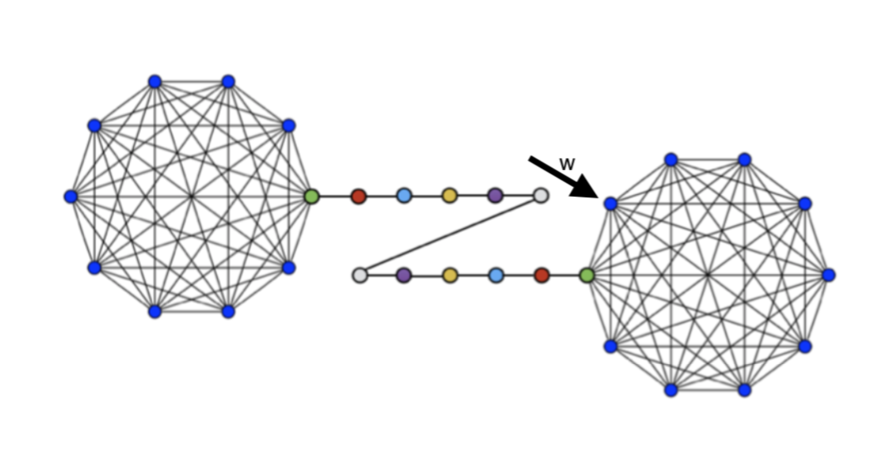
\includegraphics[width=0.6\columnwidth]{fig5.png}
		\caption{Two 10-node cliques}
		\label{fig:10-node}
	\end{figure}
	
	.\\\\\\\\
	\subsection{ node2vec \& struct2vec (ii) (3 points)}
	In the above figure \ref{fig:10-node}, suppose you arrive at node w. What are the nodes that you can reach after taking one step further with the node2vec algorithm? What about with the struct2vec algorithm (suppose that for this graph, $g_k(u, v) > 0$ for any u,v,k)?
	
	\Solution{
		\textbf{For Question 2.5:}
		
		The vector representations for the two 10-node cliques will be highly clustered and separated from each other. All 10 nodes within the left clique will have embeddings that are very close to each other, forming a distinct cluster in the embedding space. Likewise, all 10 nodes in the right clique will form another distinct cluster, located far away from the first one.
		
		No, the node embeddings from \textbf{node2vec} will not reflect structural similarity for this graph.
		
		\textbf{Justification:}
		The node2vec algorithm is based on random walks, which capture network proximity. A random walk starting in one clique is highly likely to remain within that clique for many steps before crossing the long bridge. Consequently, nodes within the same clique will co-occur frequently, resulting in similar embeddings.
		
		However, structural similarity refers to the role a node plays in its local neighborhood. A blue node in the left clique and a blue node `w` in the right clique are structurally identical: they both have a degree of 9 and are part of a 10-clique. Despite this identical structure, their embeddings will be very far apart because they belong to different communities that are distant in the graph. Therefore, node2vec captures community structure but fails to capture the identical structural roles of these nodes.
		\\\\
		\textbf{For Question 2.6:}
		
		\begin{itemize}
			\item \textbf{With node2vec:} The random walks in node2vec are performed on the original graph. From node `w` (a blue node in the right clique), there are only edges connecting it to the other 9 nodes within the same clique. Therefore, after one step, you can only reach one of the \textbf{other 9 nodes in the right-hand clique}.
			
			\item \textbf{With struct2vec:} The random walks in struct2vec are performed on a new, weighted, fully connected graph where edge weights are determined by structural similarity. Since the problem states that $g_k(u, v) > 0$ for any pair of nodes, every node is connected to every other node in this new graph. Therefore, from node `w`, you can reach \textbf{any other node in the entire graph} in a single step (with probability proportional to the structural similarity).
		\end{itemize}
	}
	
	\subsection{node2vec \& struct2vec (iii) (3 points)}
	Why is it necessary to consider different $g_k$'s during the random walk?
	(Please provide a more general answer, without limiting it to the specific example given)
	\Solution{
		It is necessary to consider different structural similarity functions $g_k$ because a node's structural role in a graph is a multi-scale concept. A single similarity function at a fixed distance $k$ provides only a limited view of this role.
		
		\begin{itemize}
			\item \textbf{Capturing Multi-Scale Roles:} Different values of $k$ capture structural patterns at different resolutions.
			\begin{itemize}
				\item A small $k$ (e.g., $k=1$) measures very local similarity by comparing the immediate neighborhoods of nodes. This can identify nodes that are centers of star-like structures or parts of local triangles.
				\item A larger $k$ measures similarity in a broader context, revealing higher-level roles. This can distinguish nodes that act as bridges between communities from nodes that are central hubs deep within a single community, even if their local neighborhoods are similar.
			\end{itemize}
			
			\item \textbf{Creating Robust Embeddings:} Two nodes might appear structurally similar at one scale but very different at another. Relying on a single $g_k$ could lead to misleading embeddings. By performing random walks that consider different $g_k$'s, the algorithm is forced to learn an embedding that integrates information from all these different structural perspectives.
			
			\item \textbf{Hierarchical Understanding:} Using a sequence of $g_1, g_2, ..., g_K$ allows struct2vec to build a hierarchical representation of structural similarity. The random walks explore a layered graph where each layer corresponds to a different scale of similarity. This process creates rich embeddings that encode a comprehensive signature of a node's structural identity across local, regional, and more global contexts.
		\end{itemize}
		In essence, using different $g_k$'s is analogous to analyzing an image at multiple zoom levels; it allows the algorithm to capture both the fine-grained details and the broader structural patterns, resulting in a much more powerful and accurate representation of a node's role.
	}
	
	\subsection{node2vec \& struct2vec (iv) (3 points)}
	Characterize the vector representations (i.e. the embedding space) of the two 10-node cliques after running the struct2vec algorithm on the graph in the above figure (Figure \ref{fig:10-node}).
	
	\Solution{
		After running the \textbf{struct2vec} algorithm, the vector representations of the nodes will be clustered based on their structural roles, completely ignoring their community membership.
		
		Specifically, the embedding space will be characterized as follows:
		\begin{itemize}
			\item All 18 "blue" nodes (9 from the left clique and 9 from the right clique) will have very similar embeddings, forming a single, tight cluster.
			\item The two "green" nodes that connect the cliques to the bridge will also have similar embeddings to each other, forming a separate cluster that is distinct from the cluster of blue nodes.
			\item The other nodes on the bridge will form their own clusters based on their respective symmetric structural roles.
		\end{itemize}
		
		\textbf{Justification:}
		The struct2vec algorithm computes similarity based on the structure of a node's local neighborhood (e.g., the distribution of degrees), not its proximity to other nodes. In the given graph, all 18 blue nodes are structurally identical; they each have a degree of 9 and are connected to 9 other nodes within a fully connected component. The algorithm will recognize this identical role and assign a high structural similarity score to every pair of blue nodes, regardless of which clique they belong to.
		
		Consequently, in the new weighted graph that struct2vec constructs for its random walks, the edges between all these blue nodes will have high weights. The random walks will frequently jump between structurally similar nodes, leading to them having nearly identical embeddings. This is in stark contrast to node2vec, which would produce two separate clusters based on the two distinct communities.
	}
	
	
	
	% Last used - Aut2324
	\section{GCN (11 points)}
	
	Consider a graph $G = (V, E)$, with node features $x(v)$ for each $v \in V$. For each node $v \in V$, let $h^{(0)}_v = x(v)$ be the node’s initial embedding. At each iteration $k$, the embeddings are updated as 
	
	$$
	\begin{aligned}
		h_{\mathcal{N}(v)}^{(k)} & =\operatorname{AGGREGATE}\left(\left\{h_u^{(k-1)}, \forall u \in \mathcal{N}(v)\right\}\right) \\
		h_v^{(k)} & =\operatorname{COMBINE}\left(h_v^{(k-1)}, h_{\mathcal{N}(v)}^{(k)}\right),
	\end{aligned}
	$$
	
	\noindent for some functions $\operatorname{AGGREGATE}(\cdot)$ and $\operatorname{COMBINE}(\cdot)$. Note that the argument to the $\operatorname{AGGREGATE}(\cdot)$ function, ${h^{(k-1)}_u, \forall u \in \mathcal{N}(v)}$, is a \textit{multi-set}.
	That is, since multiple nodes can have the same embedding, the same element can occur in ${h^{(k-1)}_u, \forall u \in \mathcal{N}(v)}$ multiple times.
	Finally, a graph itself may be embedded by computing some function applied to the multi-set of all the node embeddings at some final iteration $K$, which we notate as 
	
	$$\operatorname { READOUT }\left(\left\{h_v^{(K)}, \forall v \in V\right\}\right)$$
	
	We want to use the graph embeddings above to test whether two graphs $G_1 = (V_1, E_1)$ and $G_2 = (V_2, E_2)$ are \textit{isomorphic}.
	Recall that this is true if and only if there is some bijection $\phi : V_1 \rightarrow V_2$ between nodes of $G_1$ and nodes of $G_2$ such that for any $u, v \in V_1$, 
	$$(u, v) \in E_1 \Leftrightarrow (\phi(u), \phi(v)) \in E_2$$
	
	The way we use the model above to test isomorphism is the following. For the two graphs, if their readout functions differ, that is 
	
	$$\operatorname { READOUT }\left(\left\{h_v^{(K)}, \forall v \in V_1\right\}\right) \neq \operatorname { READOUT }\left(\left\{h_v^{(K)}, \forall v \in V_2\right\}\right),$$
	
	we conclude the graphs are \textit{not} isomorphic. Otherwise, we conclude the graphs are isomorphic. Note that this algorithm is not perfect: graph isomorphism is thought to be hard! Below, we will explore the expressiveness of these graph embeddings. 
	
	\subsection{Isomorphism Check (2 points)}
	Are the following two graphs isomorphic? If so, demonstrate an isomorphism
	between the sets of vertices. To demonstrate an isomorphism between two
	graphs, you need to find a 1-to-1 correspondence between their nodes and edges.
	If these two graphs are not isomorphic, prove it by finding a structure (node
	and/or edge) in one graph which is not present in the other. 
	\begin{figure}[H]
		\centering
		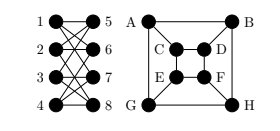
\includegraphics[width=0.5\textwidth]{fig1.png}
		\label{fig:my_label2}
	\end{figure}
	
	\Solution{
		The two graphs are \textbf{not isomorphic}.
		\\
		\\
		To prove that two graphs are not isomorphic, we need to find a graph invariant—a structural property—that differs between them. A fundamental invariant is the degree of the nodes. An isomorphism requires a one-to-one mapping of nodes that preserves adjacency, which implies that the degree of any node in the first graph must be equal to the degree of its corresponding node in the second graph.
		
		\begin{itemize}
			\item \textbf{Left Graph (Complete Bipartite Graph, $K_{4,4}$):}
			Every node in this graph has a degree of 4. For example, node 1 is connected to nodes 5, 6, 7, and 8. The degree sequence for this graph is $\{4, 4, 4, 4, 4, 4, 4, 4\}$.
			
			\item \textbf{Right Graph (Cubical Graph):}
			Every node in this graph has a degree of 3. For example, node A is connected to nodes B, C, and G. This is a 3-regular graph, and its degree sequence is $\{3, 3, 3, 3, 3, 3, 3, 3\}$.
		\end{itemize}
		
		Since the degree of every node in the left graph is 4, while the degree of every node in the right graph is 3, no degree-preserving mapping between the nodes can exist. Therefore, the graphs are not isomorphic.
	}
	
	
	\subsection{Aggregation Choice (3 points)} 
	The choice of the $\operatorname{AGGREGATE(\cdot)}$ is important for the expressiveness of the model above. Three common choices are: $$
	\begin{aligned}
		\operatorname{AGGREGATE}_{\max }\left(\left\{h_u^{(k-1)}, \forall u \in \mathcal{N}(v)\right\}\right)_i & =\max _{u \in \mathcal{N}(v)}\left(h_u^{(k-1)}\right)_i \text { (element-wise max)} \\
		\operatorname{AGGREGATE}_{\text {mean}}\left(\left\{h_u^{(k-1)}, \forall u \in \mathcal{N}(v)\right\}\right) & =\frac{1}{|\mathcal{N}(v)|} \sum_{u \in \mathcal{N}(v)}\left(h_u^{(k-1)}\right) \\
		\operatorname{AGGREGATE}_{\text {sum}}\left(\left\{h_u^{(k-1)}, \forall u \in \mathcal{N}(v)\right\}\right) & =\sum_{u \in \mathcal{N}(v)}\left(h_u^{(k-1)}\right)
	\end{aligned}
	$$
	Give an example of two graphs $G_1 = (V_1, E_1)$ and $G_2 = (V_2, E_2)$ and their initial node features, such that for some node $v_1 \in V_1$ and some node $v_2 \in V_2$ with the same initial features $h^{(0)}_{v_1} = h^{(0)}_{v_2}$, the updated features $h^{(1)}_{v_1}$ and $h^{(1)}_{v_2}$ are equal if we use mean and max aggregation, but different if 
	we use sum aggregation.\\
	\textbf{Hint:} Your node features can be scalars rather than vectors, i.e. one dimensional node features instead of n-dimensional. Also, You are free to arbitrarily choose the number of nodes (e.g. 3 nodes), their connections (i.e. edges between
	nodes) in your example.
	
	\Solution{
		Let's construct two simple graphs, $G_1$ and $G_2$, using scalar initial features. Let the target nodes be $v_1 \in V_1$ and $v_2 \in V_2$.
		
		\textbf{Graph Construction and Initial Features:}
		\begin{itemize}
			\item \textbf{Graph $G_1$:} Let node $v_1$ have two neighbors, $u_1$ and $u_2$.
			\begin{itemize}
				\item Initial features: $h^{(0)}_{v_1} = 0$, $h^{(0)}_{u_1} = 2$, $h^{(0)}_{u_2} = 4$.
				\item The multiset of neighbor features for $v_1$ is $\{2, 4\}$.
			\end{itemize}
			\item \textbf{Graph $G_2$:} Let node $v_2$ have three neighbors, $w_1$, $w_2$, and $w_3$.
			\begin{itemize}
				\item Initial features: $h^{(0)}_{v_2} = 0$, $h^{(0)}_{w_1} = 2$, $h^{(0)}_{w_2} = 3$, $h^{(0)}_{w_3} = 4$.
				\item The multiset of neighbor features for $v_2$ is $\{2, 3, 4\}$.
			\end{itemize}
		\end{itemize}
		The condition that the target nodes have the same initial features, $h^{(0)}_{v_1} = h^{(0)}_{v_2} = 0$, is satisfied. We assume a simple combine function, e.g., addition, so the difference in updated features will be driven by the aggregation step.
		
		\textbf{Aggregation Results:}
		
		\begin{enumerate}
			\item \textbf{Using Mean Aggregation:}
			\begin{itemize}
				\item For $v_1$: $h^{(1)}_{v_1} \propto \frac{1}{2}(2+4) = 3$
				\item For $v_2$: $h^{(1)}_{v_2} \propto \frac{1}{3}(2+3+4) = 3$
			\end{itemize}
			The aggregated features are \textbf{equal}.
			
			\item \textbf{Using Max Aggregation:}
			\begin{itemize}
				\item For $v_1$: $h^{(1)}_{v_1} \propto \max(\{2, 4\}) = 4$
				\item For $v_2$: $h^{(1)}_{v_2} \propto \max(\{2, 3, 4\}) = 4$
			\end{itemize}
			The aggregated features are \textbf{equal}.
			
			\item \textbf{Using Sum Aggregation:}
			\begin{itemize}
				\item For $v_1$: $h^{(1)}_{v_1} \propto 2+4 = 6$
				\item For $v_2$: $h^{(1)}_{v_2} \propto 2+3+4 = 9$
			\end{itemize}
			The aggregated features are \textbf{different}.
		\end{enumerate}
		
		This example shows that sum aggregation can distinguish between these two local neighborhood structures, while mean and max aggregation cannot, making sum aggregation more expressive in this case.
	}
	
	
	\subsection{Weisfeiler-Lehman Test (6 points)}
	Our isomorphism-test algorithm is known to be at most as powerful as the well-known \textit{Weisfeiler-Lehman test} (WL test). At each iteration, this algorithm updates the representation of each node to be the set containing its previous representation and the previous representations of all its neighbors. The full algorithm is below.
	
	\begin{figure}[H]
		\centering
		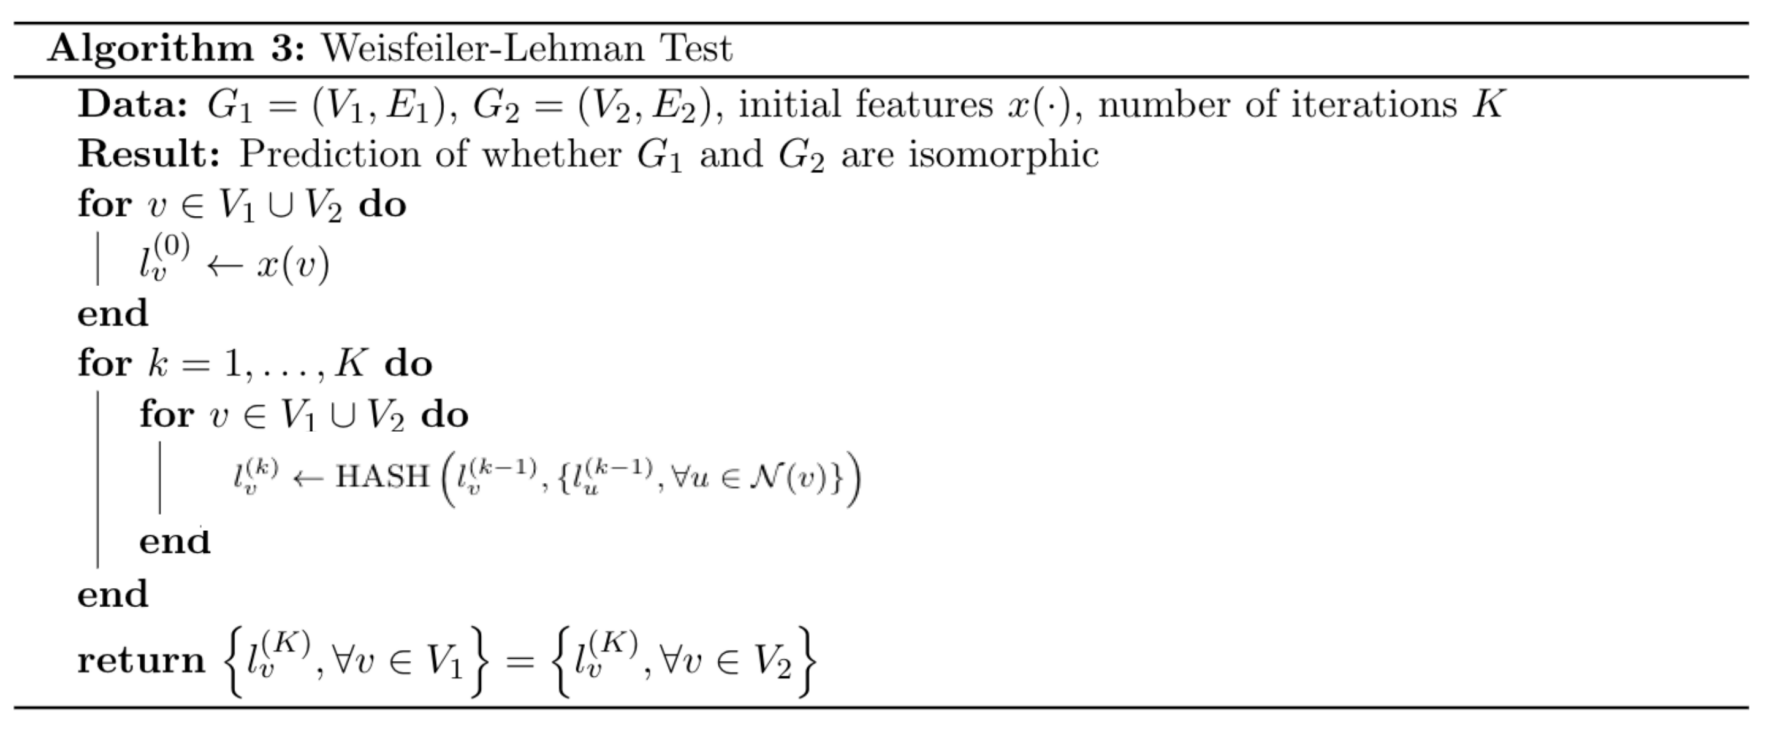
\includegraphics[width=1.0\textwidth]{algo-3.png}
		\label{fig:my_label}
	\end{figure}
	
	Prove that our neural model is at most as powerful as the WL test. More precisely, let $G_1$ and $G_2$ be non-isomorphic, and suppose that their node embeddings are updated over $K$ iterations with the same $\operatorname{AGGREGATE}(\cdot)$ and $\operatorname{COMBINE}(\cdot)$ functions. Show that if
	
	$$\operatorname { READOUT }\left(\left\{h_v^{(K)}, \forall v \in V_1\right\}\right) \neq \operatorname { READOUT }\left(\left\{h_v^{(K)}, \forall v \in V_2\right\}\right),$$
	
	then the WL test also decides the graphs are not isomorphic.\\
	
	Note: The proof has to be generic to any AGGREGATE, COMBINE, READOUT functions. Namely, it's not sufficient to show this for a specific instance of the GNN model.\\
	
	\textbf{Hint:} You can use proof by contradiction by first assuming that \textit{Weisfeiler-Lehman} test cannot decide whether $G_1$ and $G_2$ are isomorphic at the end of $K$’th iteration. Additionally, you may assume that we can choose a hash function that will not have any collisions.
	
	\Solution{
		We will prove the statement by proving its contrapositive: If the Weisfeiler-Lehman (WL) test cannot distinguish between two graphs $G_1$ and $G_2$ after $K$ iterations, then our neural model also cannot distinguish between them.
		
		\begin{enumerate}
			\item \textbf{Assumption:} Assume the WL test fails to distinguish $G_1 = (V_1, E_1)$ and $G_2 = (V_2, E_2)$ after $K$ iterations. By definition, this means that for every iteration $k \in \{0, 1, \dots, K\}$, the multiset of node "colors" (or labels) produced by the WL algorithm is identical for both graphs. This implies the existence of a bijection $\phi_k: V_1 \rightarrow V_2$ for each iteration $k$, such that for any node $v \in V_1$, its color is the same as its mapped counterpart in $G_2$:
			\[ c_v^{(k)} = c_{\phi_k(v)}^{(k)} \]
			
			\item \textbf{Inductive Proof on Embeddings:} We will now show by induction that if two nodes share the same WL color at any iteration $k \le K$, their GNN embeddings must also be identical.
			
			\textbf{Claim:} For any $k \in \{0, \dots, K\}$, if $c_v^{(k)} = c_w^{(k)}$ for $v \in V_1, w \in V_2$, then $h_v^{(k)} = h_w^{(k)}$.
			
			\begin{itemize}
				\item \textbf{Base Case (k=0):} At initialization, all nodes in the WL test have the same color, $c^{(0)}$. Similarly, in the GNN, all nodes are initialized with the same feature vector, $h^{(0)}$. Thus, the claim holds.
				
				\item \textbf{Inductive Hypothesis:} Assume the claim is true for iteration $k-1$. That is, for any pair of nodes $u_1 \in V_1, u_2 \in V_2$, if $c_{u_1}^{(k-1)} = c_{u_2}^{(k-1)}$, then $h_{u_1}^{(k-1)} = h_{u_2}^{(k-1)}$.
				
				\item \textbf{Inductive Step:} Let $v \in V_1$. From our initial assumption, there exists a node $w = \phi_k(v) \in V_2$ such that $c_v^{(k)} = c_w^{(k)}$. The WL update rule is $c_v^{(k)} = \text{HASH}(c_v^{(k-1)}, \{c_u^{(k-1)} \mid u \in \mathcal{N}(v)\})$. Since the hashes are equal and we assume no collisions, their arguments must be identical. This implies two facts:
				\begin{enumerate}[(i)]
					\item $c_v^{(k-1)} = c_w^{(k-1)}$
					\item The multiset of neighbor colors is identical: $\{c_u^{(k-1)} \mid u \in \mathcal{N}(v)\} = \{c_z^{(k-1)} \mid z \in \mathcal{N}(w)\}$
				\end{enumerate}
				Now, by our Inductive Hypothesis, these facts about colors imply facts about embeddings:
				\begin{itemize}
					\item From (i): $h_v^{(k-1)} = h_w^{(k-1)}$.
					\item From (ii): The multisets of neighbor embeddings are also identical: $\{h_u^{(k-1)} \mid u \in \mathcal{N}(v)\} = \{h_z^{(k-1)} \mid z \in \mathcal{N}(w)\}$.
				\end{itemize}
				The GNN updates the embedding for $v$ as $h_v^{(k)} = \operatorname{COMBINE}(h_v^{(k-1)}, \operatorname{AGGREGATE}(\{h_u^{(k-1)}\}))$. Since the arguments to the deterministic functions $\operatorname{AGGREGATE}$ and $\operatorname{COMBINE}$ are identical for nodes $v$ and $w$, their outputs must be identical. Therefore, $h_v^{(k)} = h_w^{(k)}$. This completes the induction.
			\end{itemize}
			
			\item \textbf{Final Readout:}
			Our inductive proof shows that if the WL test fails after $K$ iterations, there exists a bijection $\phi_K$ such that $h_v^{(K)} = h_{\phi_K(v)}^{(K)}$ for all $v \in V_1$. This means the multiset of final node embeddings for $G_1$, $\{h_v^{(K)}, \forall v \in V_1\}$, is identical to the multiset of final embeddings for $G_2$.
			
			Since the $\operatorname{READOUT}$ function is deterministic and is applied to identical multisets, the final graph embeddings must be equal:
			\[ \operatorname{READOUT}\left(\left\{h_v^{(K)}, \forall v \in V_1\right\}\right) = \operatorname{READOUT}\left(\left\{h_v^{(K)}, \forall v \in V_2\right\}\right) \]
			This shows that the GNN model also fails to distinguish the graphs.
		\end{enumerate}
		
		We have proven the contrapositive statement. Therefore, the original statement must be true: if the neural model distinguishes two graphs, the WL test must also distinguish them. This proves that the expressive power of this class of GNNs is at most that of the WL test.
	}
	
	
\end{document}





